\documentclass{article}
\usepackage[a4paper, margin=3cm]{geometry}
\usepackage[utf8]{inputenc}
\usepackage{amsmath}
\usepackage{amssymb}
\usepackage{derivative}
\usepackage[most]{tcolorbox}
\tcbuselibrary{listingsutf8}
\usepackage{graphicx}
\usepackage{float}
\usepackage{lmodern}

\title{Projet 1 : MS01}
\author{Clément Baillet et Paul Michel}
\date{}

\begin{document}
\maketitle

Voici le problème que l'on cherche à résoudre : soit $\Omega = ]0, a[ \times ]0, b[$, on cherche à calculer le champ $u(x,y)$ gouverné par
\begin{equation*}
    \left(\frac{\partial^2 u}{\partial x^2} + \frac{\partial^2 u}{\partial y^2}\right) = f(x,y), \quad \text{pour } (x,y) \in \Omega,
\end{equation*}
avec les conditions aux limites
\begin{equation*}
    u(x, 0) = U_0, \quad u(x, b) = U_0, \quad u(a, y) = U_0, \quad u(0, y) = U_0 (1 + \alpha V(y)),
\end{equation*}
pour $x \in ]0, a[$ et $y \in ]0, b[$. On suppose que $V(y) = 1 - \cos(2\pi y/b)$ et $f(x,y) = 0$, et que les paramètres $a$, $b$ et $\alpha$ sont strictement positifs, avec $\alpha < 1$. Dans toute la suite du rapport, les exemples sont réalisés pour les données suivantes : $U_0 = 1$, $\Omega = \,]0, 1[ \times \,]0, 1[$, $\alpha = 0,5$. Notre but est d'utiliser les méthodes de Jacobi et de Gauss-Seidel pour résoudre ce problème, puis de paralléliser les codes en utilisant la bibliothèque MPI, afin de les tester sur le mésocentre Cholesky.

\section{Méthode de Jacobi}

Tout d'abord, on vérifie la convergence de notre code pour $N_x = N_y = 100$ et tol$=10^{-10}$ (cf Figure \ref{fig:cvJacobi}).

\begin{figure}[H]
    \centering
    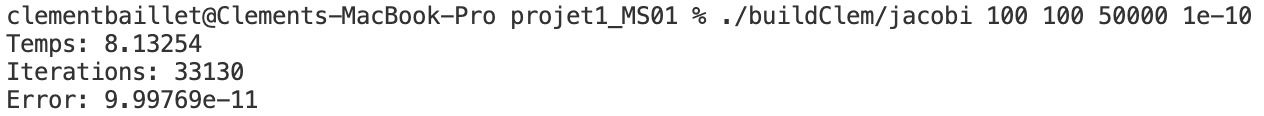
\includegraphics[width=0.9\textwidth]{cvJacobi}
    \caption{Convergence - méthode de Jacobi}
    \label{fig:cvJacobi}
\end{figure}

Pour la suite, on fixe une tolérance en précision de $10^{-6}$ ainsi qu'un nombre maximal d'itérations à $10^4$. En effectuant des tests  pour $N_x$ (respectivement $N_y$) variant dans
$$\{20,50,100,200,400,800,1600,3200,6400,12800\},$$ 
avec $N_y$ (respectivement $N_x$) fixé à $50$, on observe une tendance $Tps \propto N_x^{1,15}$ avec $R^2=0.98$ (donc très bonne régression linéaire). On note qu'on trouve $1,15$ plutôt que $1$ (complexité temporelle en $\mathcal O(N_xN_y)$ car matrice creuse).

\begin{figure}[H]
    \centering
    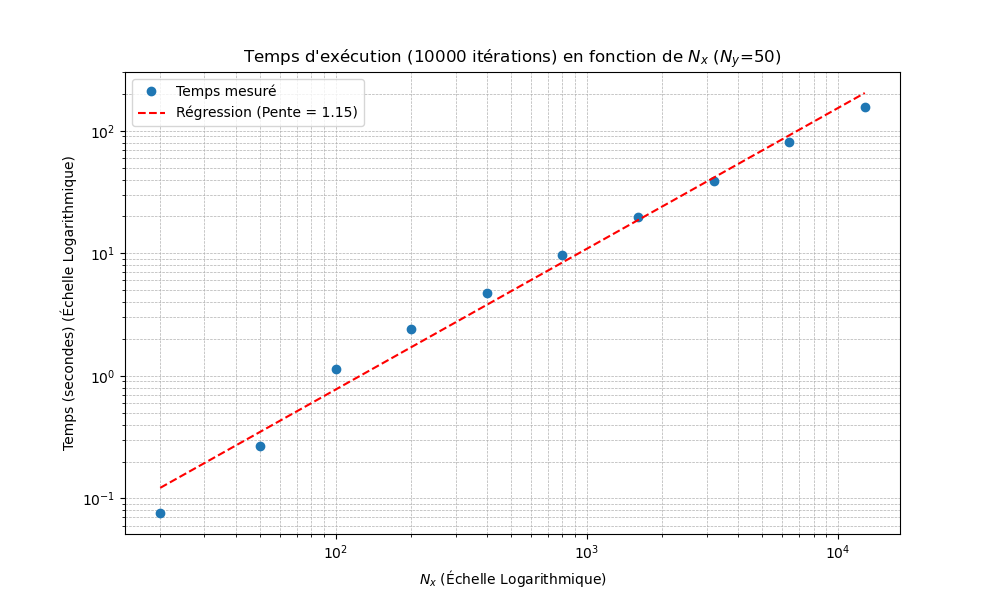
\includegraphics[width=0.9\textwidth]{courbe_log_log_jacobi.png}
    \caption{Evolution du nombre d'itérations en fonction de $N_x$ - méthode de Jacobi}
    \label{fig:loglogJacNx}
\end{figure}

\begin{figure}[H]
    \centering
    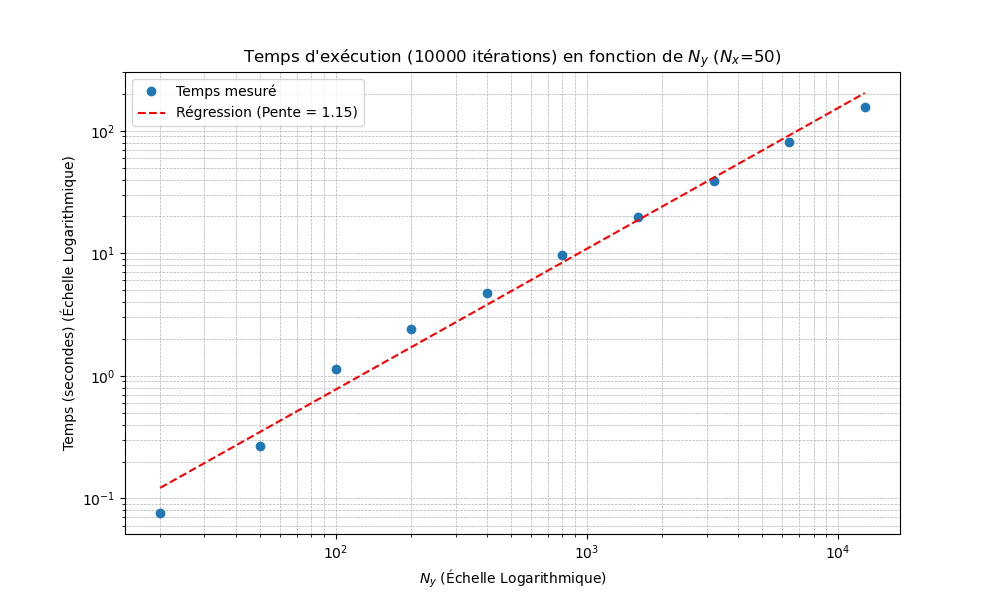
\includegraphics[width=0.9\textwidth]{courbe_log_log_jacobi_Ny.png}
    \caption{Evolution du nombre d'itérations en fonction de $N_y$ - méthode de Jacobi}
    \label{fig:loglogJacNy}
\end{figure}

\section{Méthode de Gauss-Seidel}

Comme précédemment, on vérifie la convergence de notre code pour $N_x = N_y = 100$ et tol$=10^{-10}$ (cf Figure \ref{fig:cvGS}).

\begin{figure}[H]
    \centering
    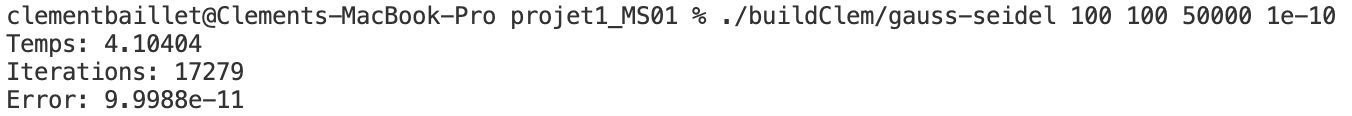
\includegraphics[width=0.9\textwidth]{cvGS}
    \caption{Convergence - méthode de Gauss-Seidel}
    \label{fig:cvGS}
\end{figure}

De même que pour Jacobi, en effectuant des tests les mêmes tests, on observe une tendance $Tps \propto N_x^{1,28}$ avec $R^2=0.98$ (donc également une très bonne régression linéaire), avec de nouveau une pente légerement différente de $1$, mais qui reste plausible.

\begin{figure}[H]
    \centering
    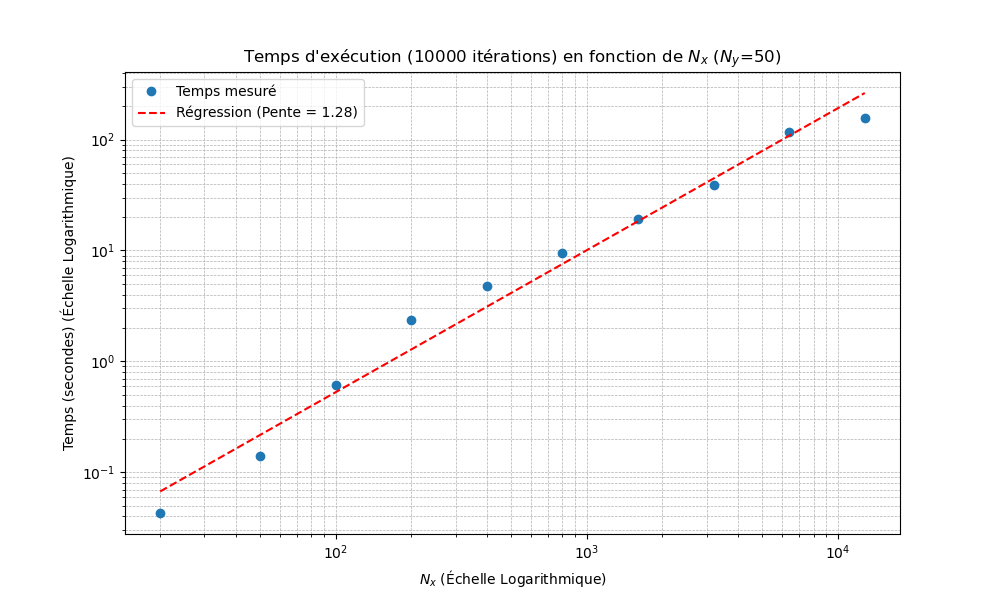
\includegraphics[width=0.9\textwidth]{courbe_log_log_gs.png}
    \caption{Evolution du nombre d'itérations en fonction de $N_x$ - méthode de Gauss-Seidel}
    \label{fig:loglogGS}
\end{figure}

\begin{figure}[H]
    \centering
    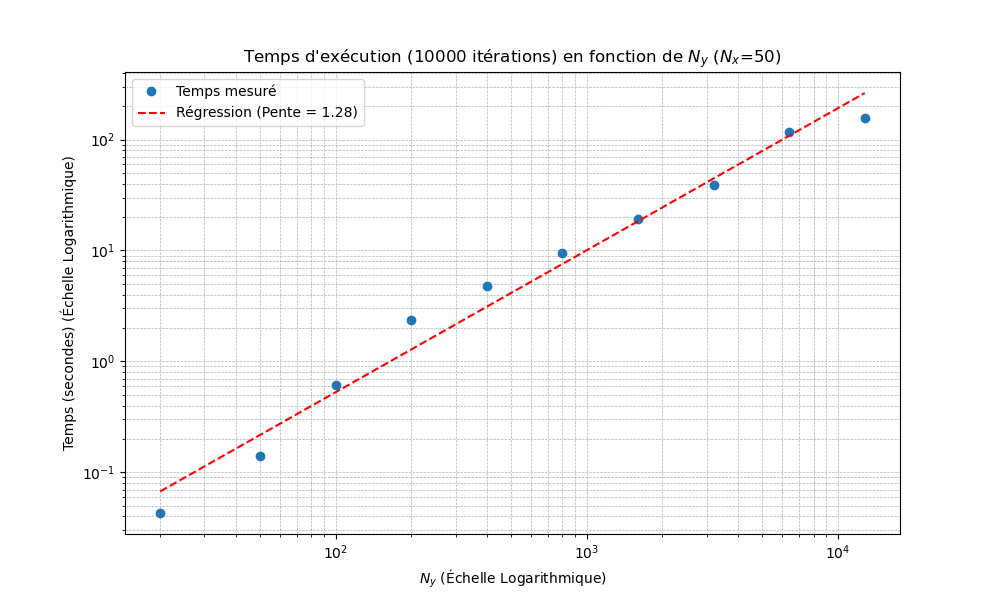
\includegraphics[width=0.9\textwidth]{courbe_log_log_gs_Ny.png}
    \caption{Evolution du nombre d'itérations en fonction de $N_y$ - méthode de Gauss-Seidel}
    \label{fig:loglogGSNy}
\end{figure}

\section{Comparaison des deux approches}
Dans la méthode de Jacobi, on met à jour $u$ à la fin de chaque boucle, alors qu'on le fait dans la boucle même pour Gauss-Seidel. Cela implique l'utilisation de 2 tableaux représentant $u$ pour Jacobi, alors qu'un seul suffit pour Gauss-Seidel. Cette observation sur le plan logique des méthodes est confirmée par la différence du nombre d'itérations avant convergence : Gauss-Seidel est une méthode presque deux fois plus rapide que celle de Jacobi en ce sens d'après les Figures $\ref{fig:cvJacobi}$ et $\ref{fig:cvGS}$. Ceci corrobore la théorie mathématique, mais nous ne la développerons pas dans ce rapport. Plus encore, en comparant le temps d'exécution entre les deux approches, on remarque une fois de plus que celle de Gauss-Seidel est légèrement plus rapide. La comparaison des deux précédentes parties sur l'évolution du nombre d'itérations en fonction de la taille de la grille se visualise sur la figure \ref{fig:comparaison}.

\begin{figure}[H]
    \centering
    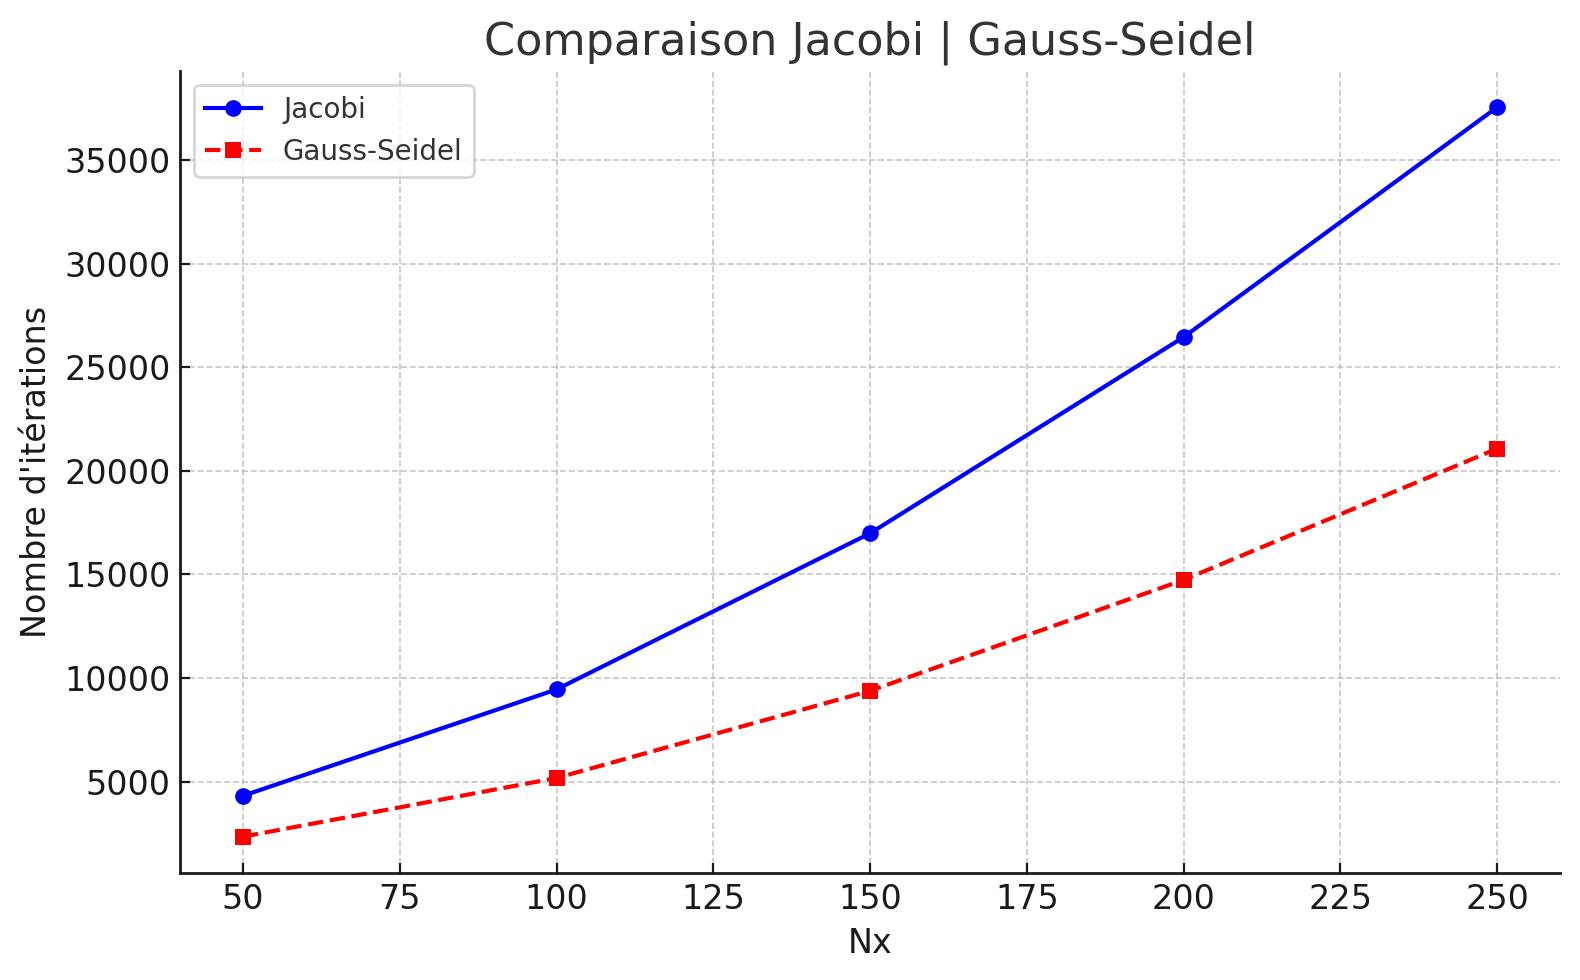
\includegraphics[width=0.9\textwidth]{comparaison_j_gs.png}
    \caption{Comparaison de l'évolution du nombre d'itérations en fonction de $N_x$}
    \label{fig:comparaison}
\end{figure}


\section{Parallélisation du code : Jacobi}

La parallélisation consiste à découper le domaine en $p$ bandes, où sur chacune d'elle, un processus s'occupe des calculs. Dans cette sous-section uniquement, les tests ont été réalisés sur une grille 500x500 avec 1 jusqu'à 6 processus sur une machine de l'ENSTA. La Figure \ref{fig:strongJac} permet l'étude de la scalabilité forte de la méthode de Jacobi.


\begin{figure}[H]
    \centering
    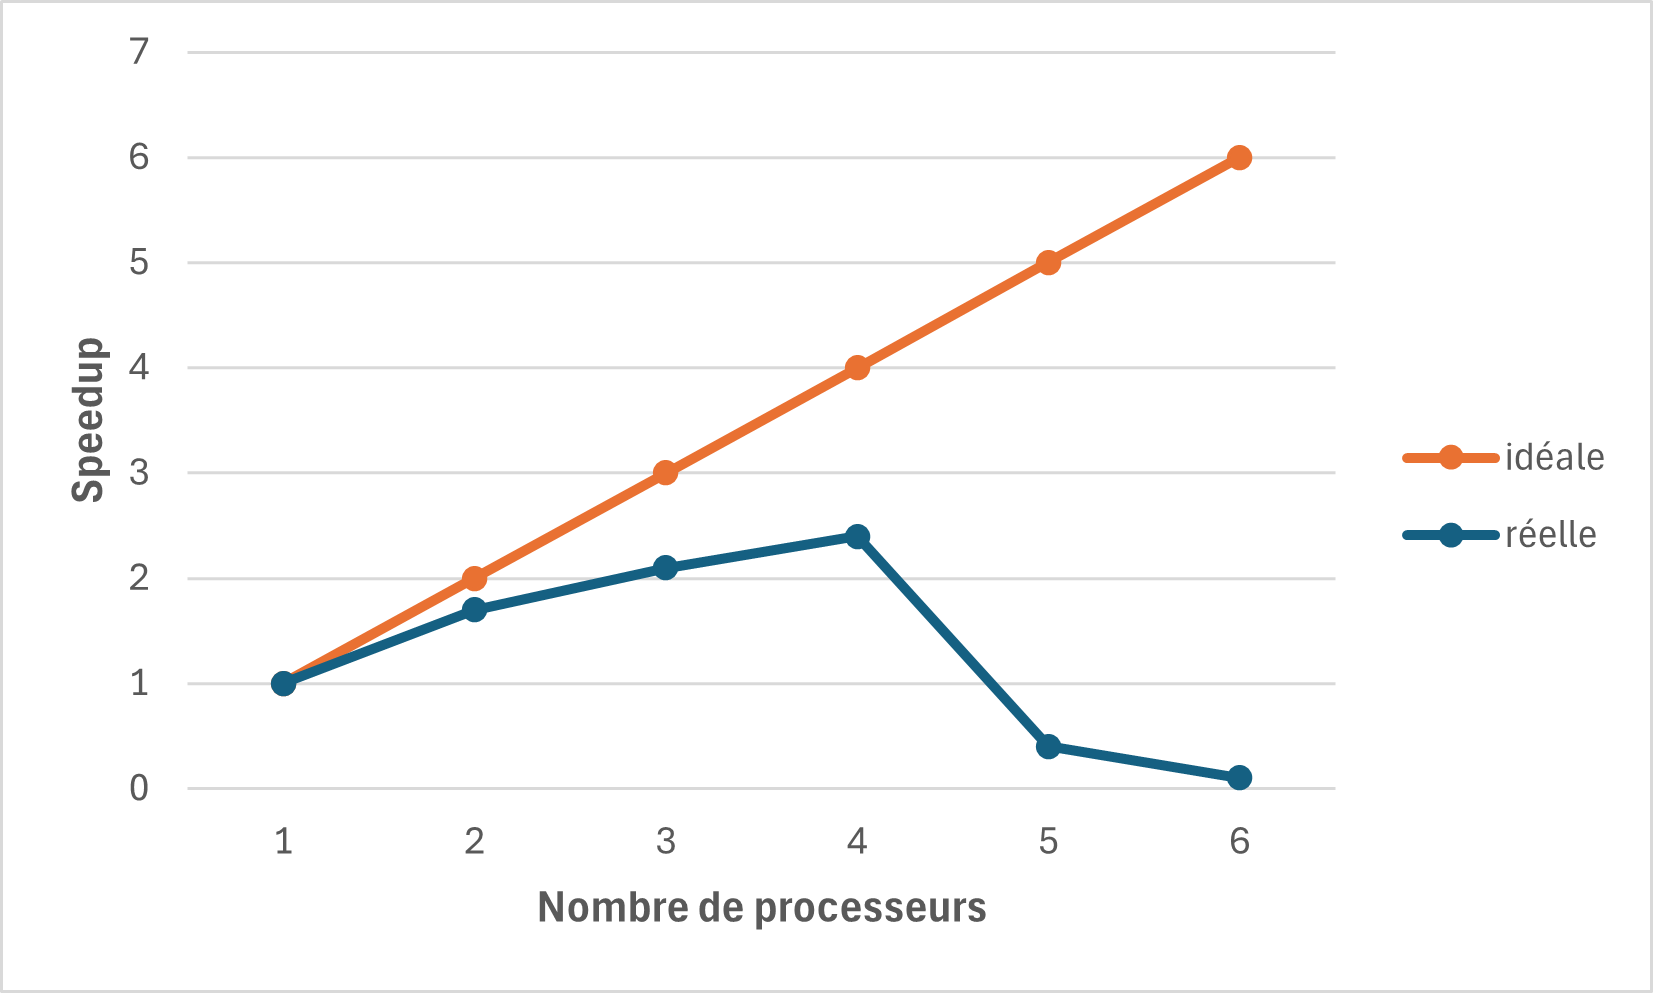
\includegraphics[width=0.9\textwidth]{strong_scaling_jacobi.png}
    \caption{Scalabilité forte - méthode de Jacobi}
    \label{fig:strongJac}
\end{figure}

On observe que le speedup croît avec le nombre de processus tant qu'on se sert de moins de 4 coeurs, limite physique du CPU après laquelle le speedup s'effondre. Sur la partie croissante, on observe une bonne scalabilité forte pour la méthode de Jacobi. On peut constater ces mêmes résultats en étudiant l'évolution de l'efficacité en fonction du nombre de processus sur la Figure \ref{fig:weakJac}.

\begin{figure}[H]
    \centering
    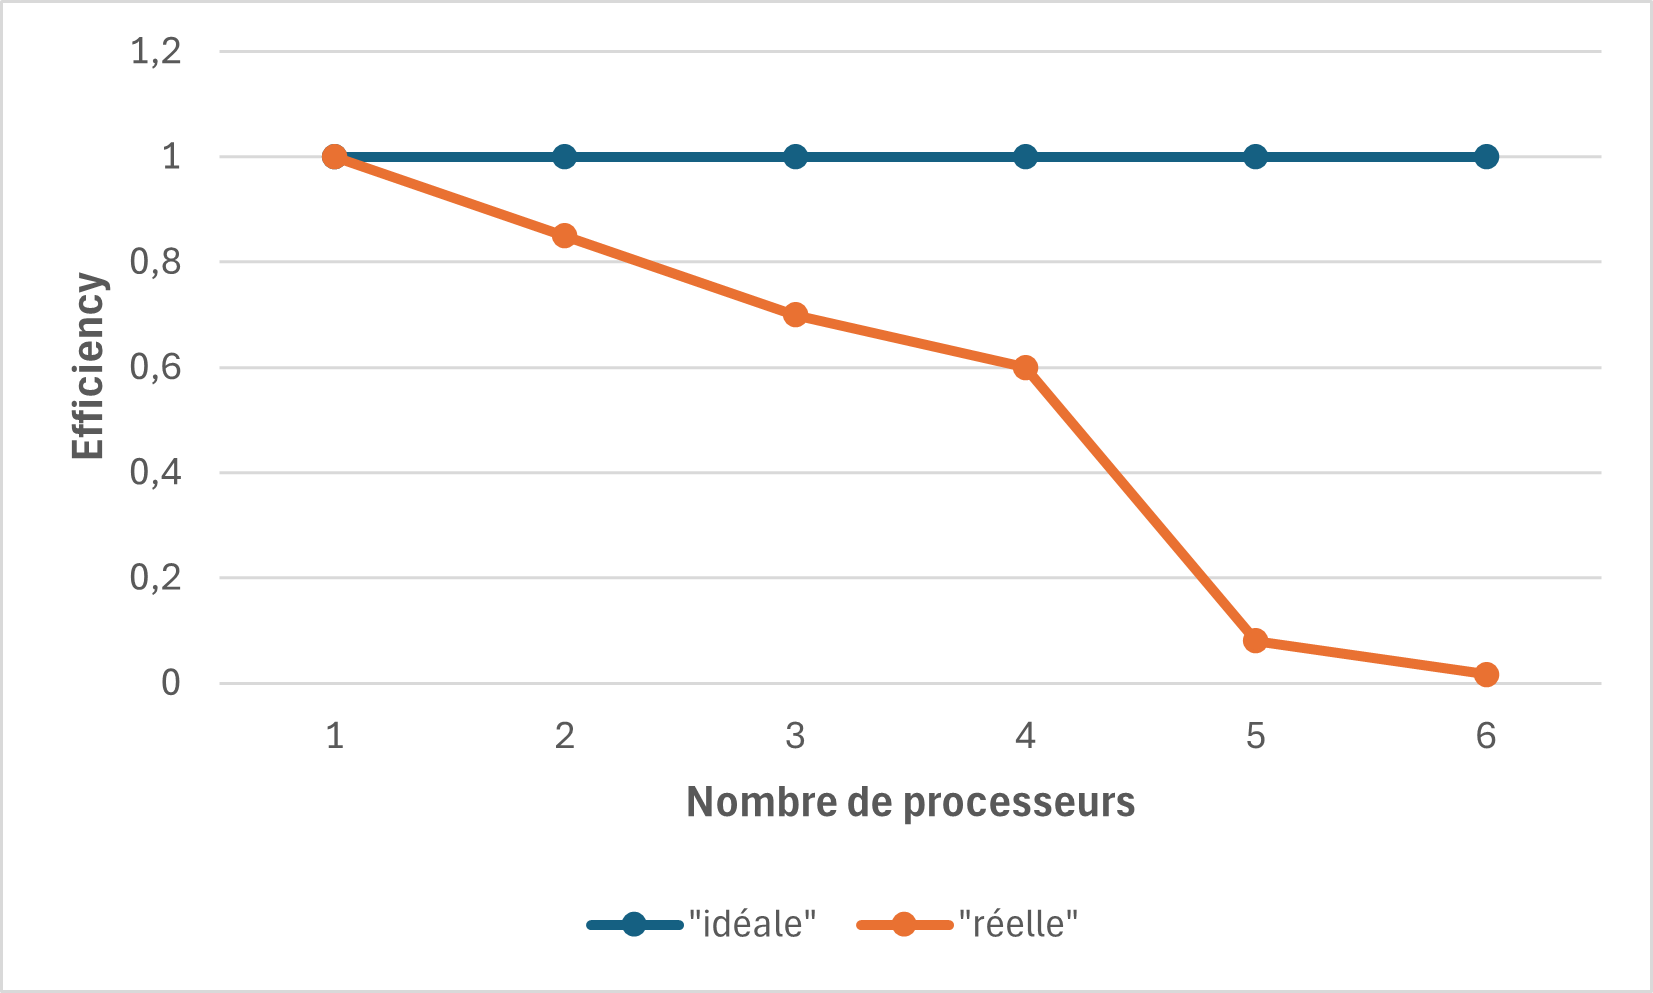
\includegraphics[width=0.9\textwidth]{weak_scaling_jacobi.png}
    \caption{Scalabilité faible - méthode de Jacobi}
    \label{fig:weakJac}
\end{figure}

Il est intéressant de remarquer qu'après avoir effectué des tests sur différentes tailles de grilles, on constate pour un petit format (50x50) un scaling moindre que pour des plus grandes grilles (300x300). Cela semble cohérent car une plus grande taille rend la parallélisation davantage intéressante.


\section{Parallélisation du code : Gauss-Seidel}


Nous avons parallélisé le code de Gauss-Seidel en utilisant la méthode dites "Rouge/Noir", qui consiste, en plus des bandes comme pour Jacobi, à découper le domaine en deux parties indépendantes dans la boucle for (une partie "Rouge" et une partie "Noire"). Bien que les différents tests aient montré que généralement Gauss-Seidel convergeait en moins d'itérations que Jacobi (idéalement 2x moins), la scalabilité forte de cette méthode est moins bonne que celle de Jacobi, notamment à cause d'un plus grand nombre de communications avec la méthode de parallélisation employée. Le graphique suivant montre les résultats obtenus pour la méthode de Gauss-Seidel et compare avec la scalabilité forte de Jacobi :

\begin{figure}[H]
    \centering
    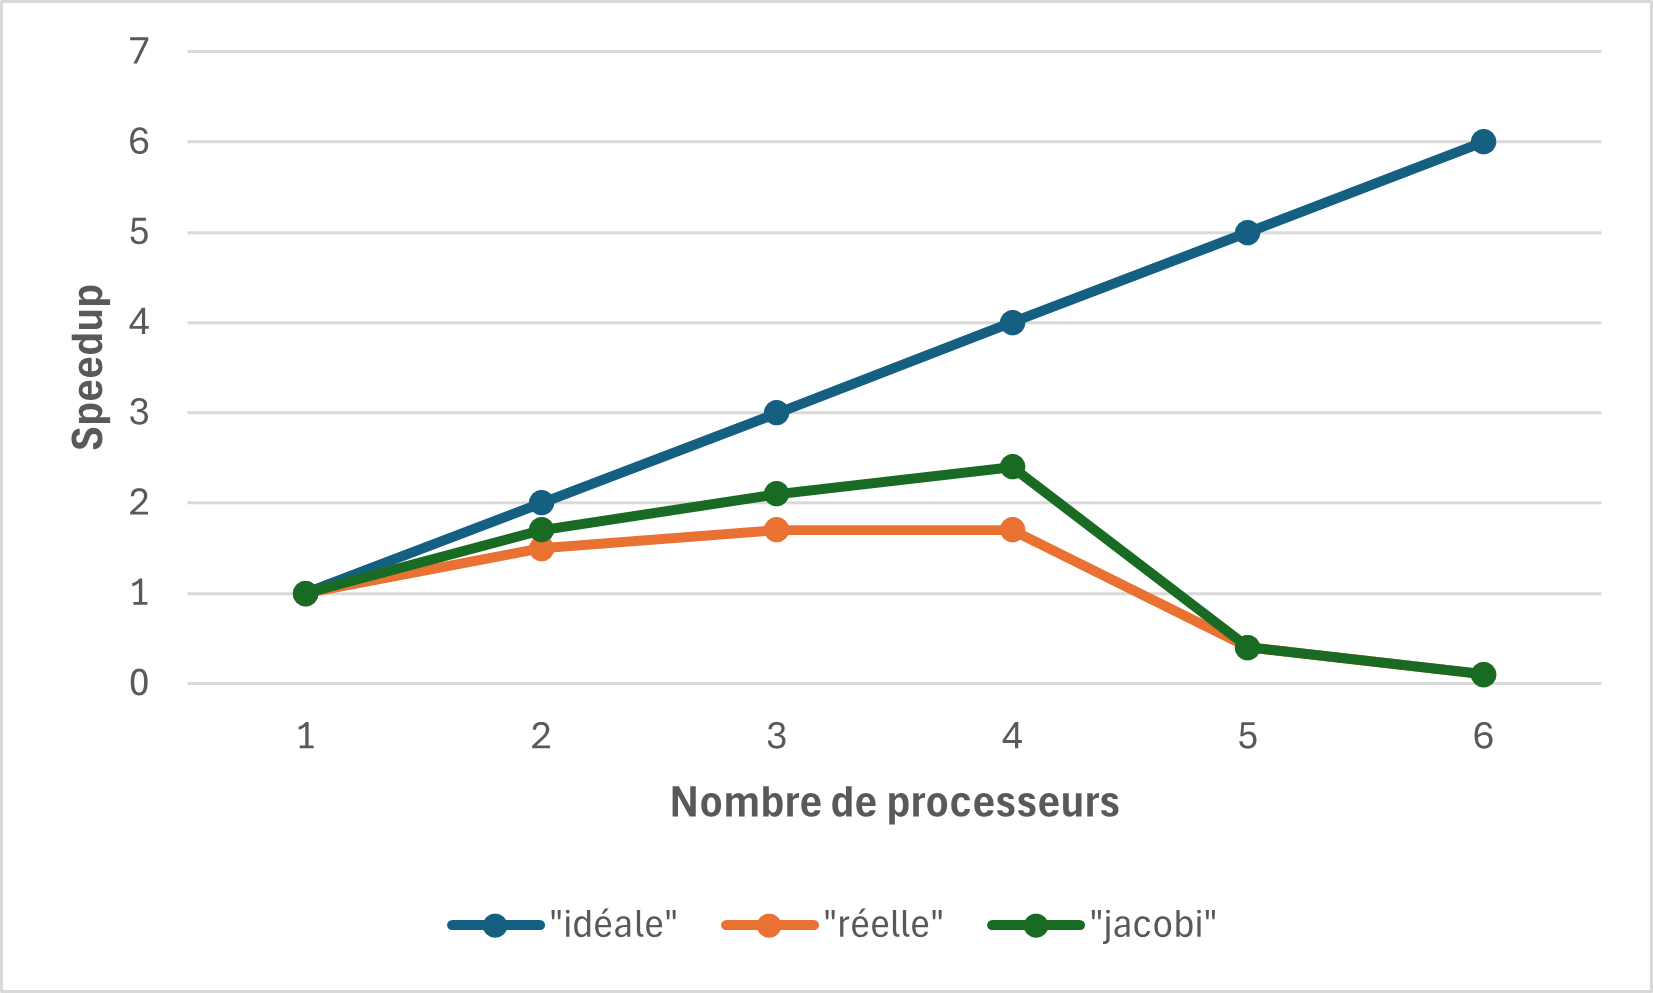
\includegraphics[width=0.9\textwidth]{strong_scaling_gs.png}
    \caption{Scalabilité forte - Gauss-Seidel et comparaison}
    \label{fig:strongGS}
\end{figure}


\section{Tests avec Cholesky}


Pour les tests sur le mésocentre Cholesky, dans un premier temps, nous avons testé la scalabilité forte pour une tolérance de $10^{-8}$, et sur un domaine fixe de $256\times 256$. Pour la scalabilité faible, nous avons augmenté progressivement la taille du domaine, en passant de $64\times 256$ à $256\times 256$. Les Figures \ref{fig:strongCholeskySmol} et \ref{fig:weakCholeskySmol} montrent les deux scalabilités avec les données obtenues.

\begin{figure}[H]
    \centering
    \includegraphics[width=0.9\textwidth]{Scalabilité_Forte_Speedup}
    \caption{Scalabilité forte - Cholesky}
    \label{fig:strongCholeskySmol}
\end{figure}

\begin{figure}[H]
    \centering
    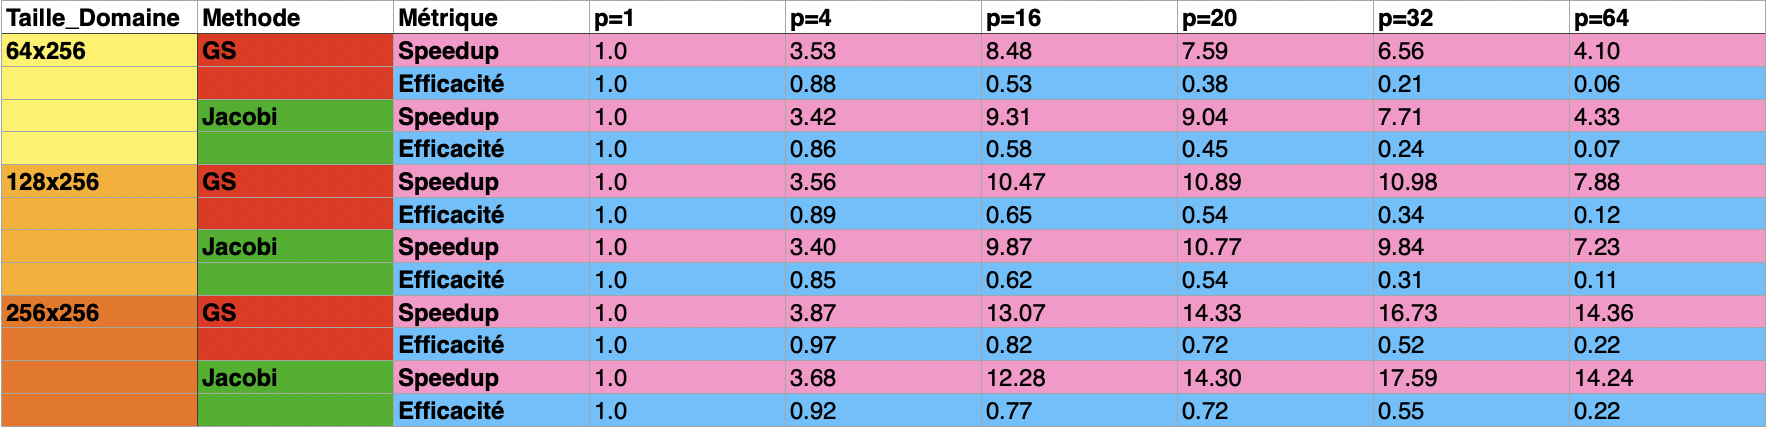
\includegraphics[width=\textwidth]{choleskySmol.png}
    \caption{Speedup et Efficacité sur petits domaines - Cholesky}
    \label{fig:weakCholeskySmol}
\end{figure}

Pour le speedup, on observe bien une augmentation quasi linéaire en fonction du nombre de processus (mais qui ne l'est pas parfaitement à cause du temps pris par les communications MPI). On note le déclin autour de $20$ processus, lié au fait que chaque noeud utilisé sur Cholesky possède $20$ coeurs. L'efficacité quant à elle, reste relativement proche de $1$ jusqu'à $20$ processus, sans l'être parfaitement à cause des communications, après quoi elle dégringole.

Dans un second temps, nous avons voulu mesurer la scalabilité faible, mais avec des domaines beaucoup plus grands: nous sommes parti d'un domaine $64\times 256$, et sommes monté progressivement jusqu'à $4096\times 256$. Malheureusement, les résultats étaient au départ très peu concluants en raison du nombre d'itérations qui explose, et qui rend l'efficacité caduque (cf Figure \ref{fig:weakCholeskyBigDom}). Nous avons donc refait une poignée de tests, en fixant cette fois-ci le nombre d'itérations maximal à $50000$. La méthode ne converge pas (et est même parfois assez loin de la tolérance fixée), mais l'efficacité est beaucoup plus proche de $1$ (avec une décroissance attendue lorsque qu'on augmente le nombre de processus, et une chute notable passé les 20 processus, cf Figure \ref{fig:weakCholeskyBigIt}).

\begin{figure}[H]
    \centering
    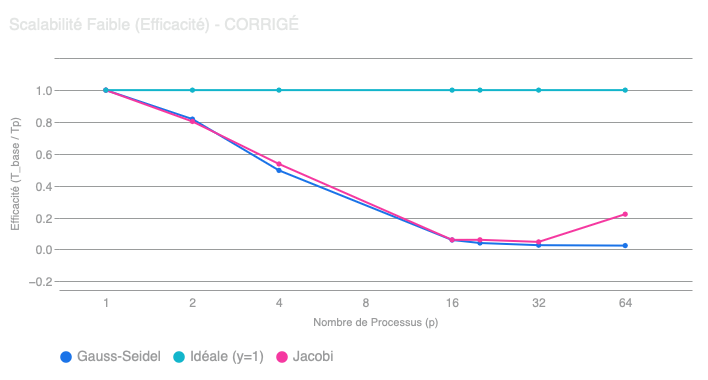
\includegraphics[width=0.8\textwidth]{Scalabilité_Faible_Efficacité}
    \caption{Scalabilité faible sur des grands domaines - Cholesky}
    \label{fig:weakCholeskyBigDom}
\end{figure}

\begin{figure}[H]
    \centering
    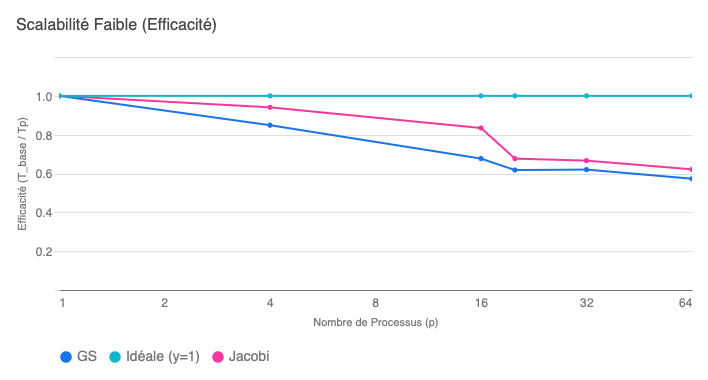
\includegraphics[width=0.8\textwidth]{Scalabilité_Faible_Efficacité_It}
    \caption{Scalabilité faible sur des grands domaines à itérations fixe - Cholesky}
    \label{fig:weakCholeskyBigIt}
\end{figure}

\section*{Conclusion}

Ce rapport compare les méthodes de Jacobi et Gauss-Seidel (GS) pour résoudre l'équation de Laplace, en séquentiel puis en parallèle avec MPI sur le cluster Cholesky.

En séquentiel, bien que Gauss-Seidel converge en deux fois moins d'itérations, l'étude de la complexité montre que Jacobi (pente 1.15) a une meilleure scalabilité que GS (pente 1.28). Ceci pourrait être dû aux opérations effectuées dans chacune des boucles, avec dans la méthode de Jacobi l'utilisation de l'itération précédente déjà entièrement calculée, et dans celle de Gauss-Seidel l'utilisation de valeurs qui viennent d'être mises à jour.

En parallèle, Jacobi (découpage en bandes) montre une meilleure scalabilité forte que GS (méthode Rouge/Noir), puisque recquiert moins d'opérations de communications. Sur Cholesky, le speedup est quasi-linéaire jusqu'à 20 cœurs (limite du nœud), mais la scalabilité faible n'est validée qu'en fixant le nombre d'itérations (et donc en compromettant la convergence).

Des potentielles pistes à suivre pour améliorer la scalabilité de ces codes, et notamment celle de Gauss-Seidel, seraient d'utiliser d'autres schémas de parallélisation, comme par exemple un schéma 2D voire 3D.

\end{document}